\chapter{Introduction}

The goal of this thesis is to describe a framework for the efficient
compilation of high-level programs into low level circuits. Also discussed will
be the use of pebble games in the optimization of reversible circuits.  A
modification to the reversible pebble game which allows for better optimization
of circuits is presented and the use of this representation as a compiler
intermediate is discussed.

\section{Landauer's principle}

This principle\cite{landauer61} states that any logical irreversible operation
must be accompanied by a corresponding entropy increase in non-information
bearing degrees of freedom. Another way of stating this is that an operation
which does not preserve information must have an associated energy cost. This
can be understood through the second law of thermodynamics which states that
the entropy of a closed system cannot decrease. That is to say that the number
of possible states in which a closed system might be cannot decrease.

The minimum bound on the amount of energy required to perform an irreversible
operation is called the Landauer limit ($kT\ln 2$).

Reversible computing shows that it is in principle possible to avoid this cost
by ensuring that no information is erased by the computation.

\section{Reversible Computation}

Normally when performing computations information is discarded. Actions such as
overwriting and clearing memory cause many states to be mapped to a single
state. So even if one had knowledge of the operations involved in a computation it
may not be possible to recover the initial state. These types of computations
are therefore called irreversible.

A computation is called reversible if any state can be traced uniquely forwards
and backwards in time, or equivalently if each step in the computation
implements a bijective function. In \cite{Bennett:73} Bennett showed that in
principle any computation could be made reversible (with a potentially large
space overhead).

Reversible computing is relevant in the context of quantum computation since it
is necessary to be able to implement unitary operations\footnote{In the
classical domain unitary operations are equivalent to reversible operations.}.
Efficient generation of quantum circuits is important since in many quantum
algorithms the cost of implementing a reversible oracle dominates\todo{cite
some evidence of this}.

The focus of this thesis is on efficiently generating the reversible parts of a
quantum computation using the circuit model. In a quantum computer conditional
operations require measurements to be made. The circuit model corresponds with
measurement free computation since all operations are applied unconditionally.
\todo{mmosca: It's still interesting of course to execute
circuits with intermediate measurements whose results we use to decide what to
do next. Your focus is on implementing the reversible pieces}

In order for an operation to be considered reversible it must be forwards and
backward deterministic\footnote{In other words it must be bijective}. For example 
Consider a classical computation where we have inputs $a$, and $b$ and wish to
know the output $a\land b$. The classical AND gate computes $(a,b)\mapsto
(a\land b)$, discarding the values of $a$ and $b$. Since this function is not
bijective (ex. $0\land 0 = 0$ and $1 \land 0 = 0$) it is not reversible.
Similarly the fanout gate $a\mapsto (a,a)$ is also not considered reversible.
This is because it is not backwards deterministic on all inputs; for example
given an input $(0,1)$ the reverse fanout gate has no defined output. 

One way to make a reversible AND operation
is to instead use the bijective function $(a,b,c) \mapsto (a,b,a\land b \oplus
c)$. This is called the ``Toffoli Gate''.  (If $c$ is initialized to zero we
have $(a,b,0) \mapsto (a,b,a\land b)$).

Any irreversible function can be made reversible using the ``Bennett
Method''\cite{Bennett:73}. In this method each irreversible gate is replaced
with a reversible version with additional space allocated as necessary. Then
the final result is copied on to the newly allocated set of bits and the entire
circuit is repeated in reverse in order to uncompute any intermediate
information computed by the circuit(see \cref{fig:bennett}). So given an irreversible
function $f(x)$ (where $f(x)$ is of size $n$) we can use the Bennett method to
generate a reversible function $(x,0^{n+m}) \mapsto (x,f(x),0^m)$.

\begin{figure}
      \capstart
      \centering
      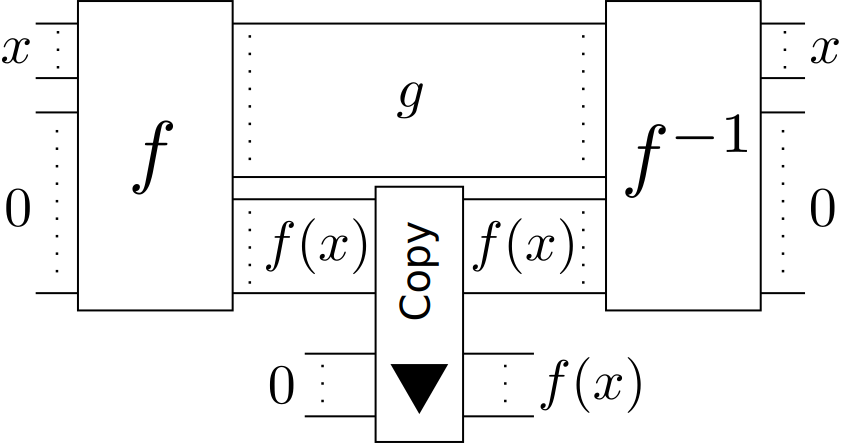
\includegraphics[width=0.8\hsize]{images/bennett}

      \caption{Bennett}

      \label{fig:bennett}
\end{figure}

The standard reversible gate set which will be used includes the following gates:

\begin{align*}
	&\text{Not:} a \mapsto \neg a \\
	&\text{Cnot:} (a,b) \mapsto (a,a\oplus b) \\
    &\text{Toffoli:} (a,b,c) \mapsto (a,b,ab\oplus c) \\
	&\text{Swap:} (a,b) \mapsto (b,a) \\
	&\text{Fredkin:} (a,b,c) \mapsto (a,\neg a b \oplus ac, ab\oplus \neg a c)
\end{align*}

Note another way of describing the Fredkin gate is as swap on $b$ and $c$
controlled on the value of $a$:

\begin{align*}
    (0,b,c) \mapsto (0,b,c)\\
    (1,b,c) \mapsto (1,c,b)
\end{align*}


\section{Quantum Circuits}

Analysis will be done using the Clifford plus T gate set.  Note that this gate
set does not include the Toffoli gate so it will have to be synthesised from
more primitive gates in the set.  This choice is made due it's availability in
error correction schemes such as the surface code\cites{}.\todo{Expand and
mention the cost of state distillation as motivation}

Long range interactions are assumed to be inexpensive in this model compared to
the cost of T gates.

\todo {Show decomposition of Toffoli gate to Clifford+T and discuss what this
means for circuit optimization.}
